\part{Appendices}
	\chapter{Terms of Reference}
	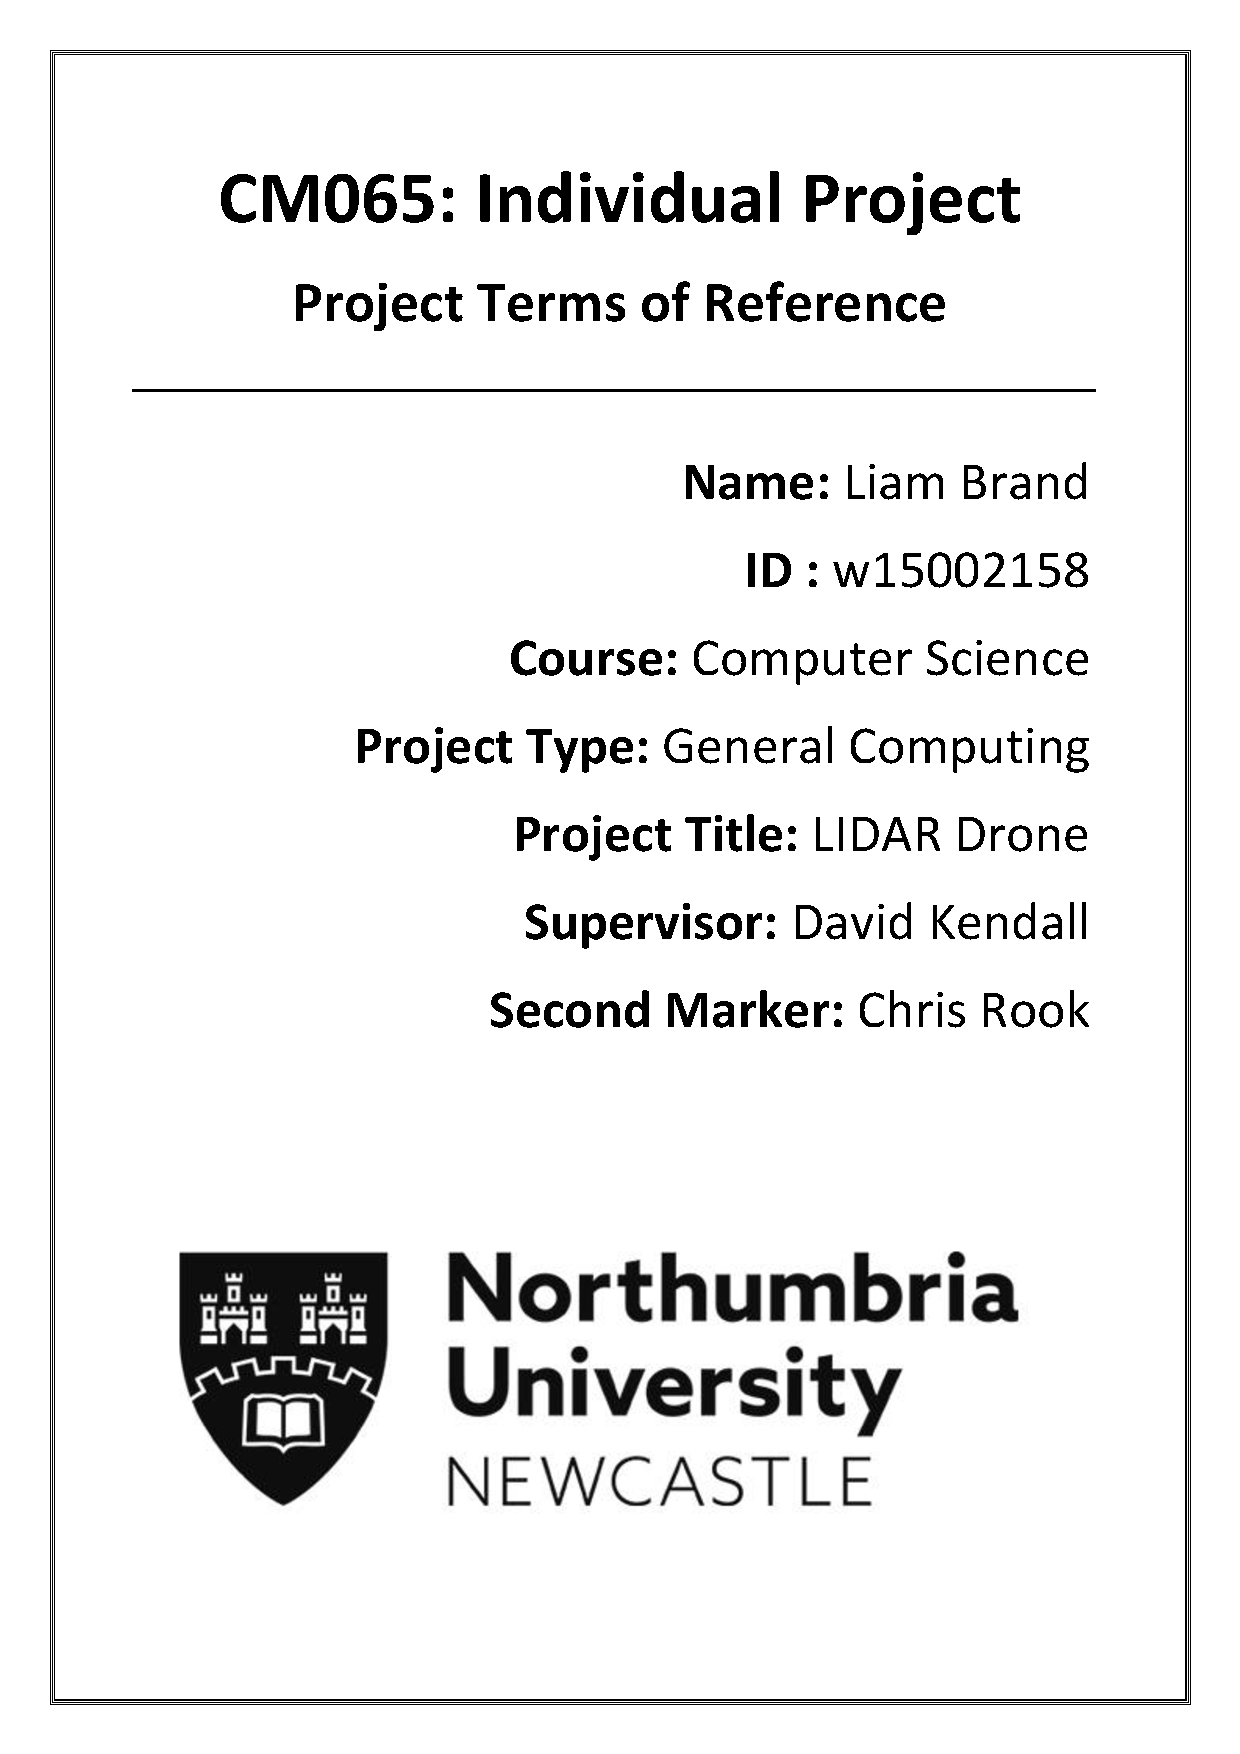
\includepdf[pages=-]{APPENDICES/TOR.pdf}
	\chapter{Testing}
	\label{testingappendices}
		\section{Tests}
		\label{testing:testlogs}
			\begin{landscape}
				\subsection{Basic Movement Tests}
				\begin{table}[h!]
					\centering
					\label{table:movementtestsbasic}
					\begin{tabular}{|| l | l ||} 
						\hline
						Printed Direction & Direction Moved In  \\ [0.5ex] 
						\hline
						Right & Right   \\
						Left & Left   \\ 
						Forward & Forward   \\ 
						Left & Left   \\ 
						Right & Right   \\ 
						Forward & Forward   \\ 
						Right & Right   \\ 
						Left & Left   \\ 
						Backward & Backward   \\ 
						Forward & Forward   \\ 
						Backward & Backward   \\ 
						Left & Left   \\ 
						Right & Right   \\ 
						Right & Right   \\ 
						Backward & Backward   \\ 
						Forward & Forward   \\ 
						Forward & Forward  \\ 
						Backward & Backward  \\ 
						Right & Right   \\ 
						Forward & Forward   \\ 
						Backward & Backward   \\ [1ex] 
						\hline
					\end{tabular}		
				\end{table}
			
				\subsection{System Test}
				\begin{table}[h!]
					\centering
					\label{systemintergrationtestingtable}
					\begin{tabular}{| p{2.5cm} | p{5cm} | p{4cm} | p{4cm} | p{1.5cm} | p{2cm} |} 
						\hline
						Test & Test Purpose & Expected Result & Actual Result & Pass/Fail & Comments \\ [0.5ex] 
						\hline
						Drive Forward & The robot should move forwards during its operation & As expected & The robot moved forwards when it was switched on & Pass & Hardcoded movement  \\
						
						Drive Right & The robot should move right during its operation & The robot is able to move right & The robot couldn't move right & Fail &   \\
						
						Drive Left & The robot should move left during its operation & The robot is able to move left & The robot couldn't move left & Fail &   \\
						
						Motor Obstructions & During the previous drive tests, there should be no obstructions to the motors from the robot's other components & As expected & The robot's motors didnt get blocked & Pass &   \\
						
						Scanning & The robot should stop to scan & The robot stops and scans its environment & As predicteda & Pass &   \\ 
						
						Write Scan Data & Ensure the robot can write scanned data to the Micro SD-Card & The Micro SD-Card will contain a file with scan data & As expected & Pass & Plugged in and viewed with USB adapter  \\
						 
						Writing Duration & Ensure the robot writes data to the Micro-SD Card in a reasonable time  & Writing should be done in under ten seconds & Writing was done in under ten seconds & Pass & Ready light flashed indicating writing task was finished  \\ 
						
						Generate Map & Using the robot's scan data, the GUI should produce a basic map & Map will be produced resembling the robot's environment & Map was produced but didn't resemble the environment & Fail &  \\ 
						
						Generate Map Without File & Make the GUI attempt to generate a map without an available file & GUI will catch and handle a runtime exception & As expected & Pass &  \\ 
						
						Map Multiple Areas & Mapping should work on multiple different environments & Each map will be accurate to the environment the robot was in & Maps didn't resemble the environment & Fail &  \\ 
						
						Repeated Mapping & Repeated maps of the same area should look similar & Map will be produced resembling the robot's environment & Maps didn't resemble the environment & Fail &  \\ 
						
						SLAM & The system should be capable of producing a dynamic map using multiple scans from different locations & The GUI creates a map from the robot's scan data & No such functionality & Fail &  \\ [1ex] 
						\hline
					\end{tabular}	
				\end{table}
			\end{landscape}

		\section{Test Code}
		\label{testing:testcode}
			\subsection{Testing the Movement}
			\label{testcode:movementbasic}
			\begin{lstlisting}
				while (true) {
					// Random number between 0 and 3
					int r = rand() % 4;
					
					if(r == 0) {
						pc.printf("Forward");
						goForward();
					}
					
					if(r == 1) {
						pc.printf("Right");
						goRight();
					}
					
					if(r == 2) {
						pc.printf("Back");
						goBackward();
					}
					
					if(r == 3) {
						pc.printf("Left");
						goLeft();
					}

					OSTimeDlyHMSM(0,0,3,0);
				}
			\end{lstlisting}
			
			\subsection{Testing the Observation}
			\label{testcode:observation1}
			\begin{lstlisting}
			static void appTaskLidarTest(void *pdata) {
				dtr = 1;
				rplidar.begin(lidar_device);
				rplidar.startScan();
				struct RPLidarMeasurement measurement;
				
				while (true) {
					rplidar.waitPoint();
					measurement = rplidar.getCurrentPoint();
					pc.printf("Distance: %f Angle:%f\n", measurement.angle, measurement.distance);
					OSTimeDlyHMSM(0,0,0,100);
				}
			}
				\end{lstlisting}
			
		
		\subsection{Testing the Observation}
